\chapter{Teoria da Medida}

Nesta seção é apresentada a teoria medida em sua forma mais elementar.
As definições e conceitos foram todas baseadas em \cite{elon}, \cite{bartle} e \cite{magalhaes}.

\section{Conjuntos Mensuráveis}
Nesta seção dedicaremos nosso estudo à entender a Teoria da Medida e da Integração de uma forma mais abrangente.
Para tal, o conceito de $\mathcal{C}$-álgebra é extremamente necessário. Assim, segundo \cite{bartle}, temos a
\index{$\mathcal{C}-$álgebra}

% Definição de Sigma álgebra
\begin{definition}
\label{def:sigma-algebra}

    Seja $X$ um conjunto não vazio. Uma família $\mathcal{C}$ de subconjuntos de $X$ é dita uma \sigal se as seguintes condições são atendidas:
    \begin{enumerate}[label*= (\roman*)]
        \item $\varnothing$ e $X$ são elementos de $\mathcal{C}$;     
        \item Se um elemento $A \in \mathcal{C}$, então $A^c \in \mathcal{C}$
        \footnote{Em todo o texto, $X^c$ significa o \textit{complementar do conjunto} $X$.};
        \item Se $(A_n)$ é uma sequência de elementos de $\mathcal{C}$, 
        então $\displaystyle \bigcup_{j = 1}^\infty A_j \in \mathcal{C}$.
    \end{enumerate}

\end{definition}

Um par ordenado $(X, \mathcal{C})$  constituído de um conjunto $X$ e uma \sigal sobre $X$ é chamado de  \textbf{espaço mensurável} . \index{espaço mensurável}
Além disso, cada elemento deste espaço é chamado de conjunto $\mathcal{C}-$mensurável.
Quando não houver confusão ou quando a \sigal estiver fixada, dizemos simplesmente que cada elemento é um conjunto mensurável.

\begin{remark}
	Em todo o texto, indicaremos por $I_n$ o conjunto dos $n$ primeiros números naturais. 
	Assim, $I_n = \{k \in \N; 1 \leq k \leq n\}$.
\end{remark}

% União finita de elemento da sigma algebra
\begin{proposition}
\label{prop:sigma-união-finita}
    Seja $\mathcal{C}$ uma \sigal de um conjunto $X$. Se $A_1, ..., A_n$ são todos elementos quaisquer de $\mathcal{C}$, então $\displaystyle \bigcup_{j = 1}^n A_j$ é um elemento de $\mathcal{C}$.
\end{proposition}
\begin{prova}
	Seja $A_1,\ldots, A_n$ elementos de $\cc$. 
	Construa uma sequência $(B_n)$ tal que $B_j = A_j$ para todo $j \in I_n$ e $A_{n + 1} = A_{n + 2} = \cdots = \varnothing$.
	Desta forma, pelo item \textit{(iii)} da definição de \sigal, temos que 
	$
	\displaystyle\bigcup_{j = 1}^\infty B_j = \bigcup_{j = 1}^n A_j
	$.
	Como $\displaystyle \bigcup_{j = 1}^\infty B_j \in \cc $ segue que 
	$\displaystyle \bigcup_{j = 1}^n A_j \in \cc $.
\end{prova}

%\begin{remark}
%	Às vezes, por praticidade, denotaremos a união enumerável infinita de uma família de elementos $(E_n)$ de uma \sigal $\cc$ como 
%	$\displaystyle \bigcup_{n \in \N} E_n$ ao invés de 
%	$\displaystyle \bigcup_{j = 1}^\infty E_n$.
%	A mesma convenção pode ser aplicada para interseção.
%\end{remark} 
% 
 
% Exemplos de Sigmas Algebras 
\begin{example}
    Seja $X = \{-1,0,-1\}$. Se considerarmos $\mathcal{C} = \{\varnothing, X, \{0\}, \{-1,1\}\}$, temos que $(X, \mathcal{C})$ é um espaço mensurável.
\end{example}

\begin{example}
\label{ex:sigma-trivial}
    Seja $X$ um conjunto qualquer.
    O conjunto $\mathcal{C}_1 = \{\varnothing, X\}$ é uma \sigal de $X$.
    De fato, podemos observar que, neste exemplo, todas as condições impostas na definição \ref{def:sigma-algebra} são atendidas de maneira trivial, pois 
    $\varnothing$ e $X$ são todos os elementos de $\mathcal{C}_1$. 
    Assim,  $(X, \mathcal{C}_1)$ é um espaço mensurável.
\end{example}

Perceba que a definição \ref{def:sigma-algebra} não nos diz que uma \sigal de um conjunto é única.
Realmente, não é. 
Assim, um conjunto pode gerar espaços mensuráveis diferentes a depender da \sigal adotada.
Para evidenciar essa percepção, observe o exemplo a seguir:

\begin{example}
	\label{ex:sigma-subconjuntos}
	Seja $X$ dado de maneira arbitrária conforme o exemplo anterior.
	Considere, agora, o conjunto $\mathcal{C}_2 = \{ A; \ A \subset X\}$, ou seja, o conjunto formado por todos os subconjuntos do conjunto $X$.
	%
	\footnote{Também chamado de conjunto das partes de $X$ e, as vezes, representado por $\mathcal{P}(X)$.}
	%
	Sabemos que $\varnothing \subset X$ e $X \subset X$. 
	Assim, $\varnothing, X \in \mathcal{C}_2$. 
	Se tomarmos um conjunto $A \subset \mathcal{C}_2$, então $A^c = X - A$ por definição.
	Ou seja, $A^c$ é formado por elementos que estão todos em $X$ caracterizando-o um elemento de $\mathcal{C}_2$.
	Da mesma forma, se tomarmos uma sequência $(A_j)$ de elementos de $\mathcal{C}_2$, a reunião 
	$\displaystyle \bigcup_{j = 1}^\infty A_j$ é composta por elementos de $X$.
	Logo,  $\displaystyle \bigcup_{j = 1}^\infty A_j \in \mathcal{C}_2$.
	Com isso, $\mathcal{C}_2$ também é uma \sigal de $X$ e o par $(X, \mathcal{C}_2)$ é um espaço mensurável que, por sua vez, é diferente do espaço $(X,\mathcal{C}_1)$.
\end{example}



% Como todo estudo de matemática, após vermos definição e exemplos precisamos aprofundar-nos na natureza do objeto que estamos estudando.
% Partindo deste ponto, vamos dar início a uma sequencia de proposições que servirão como ferramenta para caracterizações futuras dos espaços mensuráveis.

Os exemplos apresentados acima são todos de conjuntos que são uma \sigal de um conjunto $X$ arbitrário.
Por definição, o conjunto $\mathcal{C}$ é composto de subconjuntos do conjunto $X$. 
Será que se construirmos $Z$ um conjunto que contenha $\varnothing$ e $X$ e outros subconjuntos do conjunto $X$ tomados aleatoriamente teremos $(X,Z)$ um espaço mensurável? A resposta é negativa conforme o exemplo seguinte.

%Contra Exemplo
\begin{counterexample}
    Seja $X = \{x,y,z\}$. O conjunto $\mathcal{C} = \{\varnothing, X, \{x\}, \{y\}, \{z\}\}$ não é uma \sigal de X.
    Sem dúvida, $\varnothing, X \in \mathcal{C}$. 
    Entretanto, perceba que $\{x\} \in \mathcal{C}$, mas $\{x\}^c \notin \mathcal{C}$.
    De fato, $\{x\}^c =\{x,y,z\} -\{x\} = \{y,z\}$ e $\{y,z\} \notin \mathcal{C}$.
    Assim, a segunda condição da definição \ref{def:sigma-algebra} não é satisfeita impossibilitando que $\mathcal{C}$ seja uma \sigal de $X$.
    
\end{counterexample}

Por vezes, em matemática, é interessante  conseguirmos construir algum conjunto que contenha uma propriedade que desejamos. 
A proposição a seguir nos mostra como podemos fazer isso para criar uma \sigal em um conjunto.

% Assim, pode ser preciso construir uma \sigal em algum momento com um conjunto $A$ específico.
% A proposição adiante nos mostra como isso pode ser feito:

\begin{proposition}
\label{prop:sigma-complementar}
    Seja $X$ e $A$ dois conjuntos quaisquer com $A \neq \varnothing$.
    Se $A \subset X$, então o conjunto 
    $\mathcal{C}=\{\varnothing, X, A, A^c\}$ é uma \sigal de $X$.
\end{proposition}

\begin{prova}
    Perceba que as condições \textit{(i)} e \textit{(ii)} da definição \ref{def:sigma-algebra} são satisfeitas pela forma que o conjunto  $\mathcal{C}$ foi construído. Para verificar a última condição, basta perceber $A \cup A^c = X$. Assim, as sequências construídas terão comportamento análogo as do exemplo \ref{ex:sigma-subconjuntos}. Portanto, $\mathcal{C}$ é uma \sigal de $X$ para qualquer que seja $ \varnothing \neq A \subset X$.
\end{prova}

\begin{example}
    Considere $X = \N$. 
    Sejam $P =\{2k; \ k \in \N\}$ e $I = \{2k - 1;\ k \in \N\}$. 
    Como $P^c = I$, então $\mathcal{C} = \{\varnothing, \N, P, I\}$ é uma \sigal de $\N$ pela proposição anterior.
\end{example}

Observe que o conjunto $A$ que apresentamos na proposição \ref{prop:sigma-complementar} é um subconjunto não vazio do conjunto $X$ que fora tomado arbitrariamente. 
\footnote{Observe que se $A = \varnothing$, a \sigal é a mesma do exemplo \ref{ex:sigma-trivial}.}
Uma pergunta intuitiva é: se tomarmos um conjunto $A$ que não é subconjunto de $X$ o espaço $(X, \mathcal{C})$ continua sendo mensurável? A resposta é não.
Se o conjunto $A$ não for subconjunto de $X$ não temos como garantir a validade da condição \textit{(ii)}  da definição \ref{def:sigma-algebra}, pois  $A^c$ não necessariamente é subconjunto de $X$ o que não permitiria os argumentos usados anteriormente na proposição \ref{prop:sigma-complementar}. 
Dito isso, note que a definição \ref{def:sigma-algebra} e a proposição \ref{prop:sigma-união-finita} tratam apenas da união enumerável ou finita, respectivamente. A partir de agora investigaremos propriedades voltadas a interseção entre conjuntos mensuráveis.

% Propriedades de Interseção 

\begin{proposition}
\label{prop:interseção-elementos-sigmas}
    Seja $X$ um conjunto e $\mathcal{C}$ uma \sigal desse conjunto.
    Se $(A_j)$ é uma sequência  de conjuntos $\mathcal{C} $-mensuráveis, então $\displaystyle \bigcap_{j = 1}^\infty A_j$ é um elemento $\mathcal{C}$-mensurável.
\end{proposition}
\begin{prova}
    Se $A_j \in \mathcal{C}$ para todo $j \in \N$, então cada complementar $A_j^c \in \mathcal{C}$, pois $\mathcal{C}$ é $\sigma$-álgebra. 
    Assim, $(A_j^c)$ forma uma sequência de conjuntos $\mathcal{C}$-mensuráveis acarretando que 
    $\displaystyle \bigcup_{j = 1}^\infty A_j^c \in \mathcal{C}$. 
    Segue, pelas \textit{Leis de Morgan}, que 
    $$
    \displaystyle \bigcup_{j = 1}^\infty A_j^c 
    = \left(\displaystyle \bigcap_{j = 1}^\infty A_j\right)^c
  	$$
	Logo, $\left(\displaystyle \bigcap_{j = 1}^\infty A_j\right)^c \in \mathcal{C}$ o que implica $\displaystyle \bigcap_{j = 1}^\infty A_j \in \mathcal{C}$. 
	Portanto, $\displaystyle \bigcap_{j = 1}^\infty A_j$ é um conjunto $\mathcal{C}$-mensurável.
\end{prova}

Considere a \sigal apresentada na proposição \ref{prop:sigma-complementar}. 
Qualquer outra \sigal $\mathcal{F}$ que tiver $A$ como elemento, conterá $\mathcal{C}$.
Assim, observamos que 
$$
\mathcal{C} = \displaystyle \bigcap_{\mathcal{F} \supset A} \mathcal{F}.
$$
Esta \sigal $\mathcal{C}$   definimos como a \textit{menor} \sigal gerada por $A$. \index{gerada por um conjunto}
%
\footnote{Lembre que a noção de \enquote{menor} aqui é trazida por meio da relação de ordem parcial gerada pela relação de inclusão entre conjuntos.}
%
Sabendo que a menor \sigal é gerada por meio de intersecção é natural o seguinte questionamento: a interseção entre \sigals ainda é uma \sigal? Para responder à esta pergunta temos a proposição adiante.

%Interseção de Sigmas algebras
\begin{proposition}
\label{prop:interseção-2sigmas}
    Se $\mathcal{C}_1$ e $\mathcal{C}_2$ são duas \sigals de um conjunto $X$, então $\mathcal{C} = \mathcal{C}_1 \cap \mathcal{C}_2$ também é uma \sigal do conjunto $X$.
\end{proposition}

\begin{prova}
    Se $\mathcal{C}_1$ e $\mathcal{C}_2$ são \sigals de $X$, então ambos possuem $\varnothing$ e $X$ como elementos.
    Assim, $\varnothing$ e $X$ estão na intersecção $\mathcal{C}$.
    Além disso, se $A \in \mathcal{C}$, então $A \in \mathcal{C}_1$ e $A \in \mathcal{C}_2$. 
    Por serem ambas \sigals, $A^c \in \mathcal{C}$ e $A^c \in \mathcal{C}_2$.
    Ou seja, $A^c \in \mathcal{C}_1 \cap \mathcal{C}_2 = \mathcal{C}$.
    Por fim, se tomarmos uma sequência $(A_n)$ de elementos de $\mathcal{C}$, observamos que $A_j \in \mathcal{C}_1$ e $A_j \in \mathcal{C}_2$ para cada $j \in \N$.
    Assim, $\displaystyle \bigcup_{j = 1}^\infty A_j \in \mathcal{C}_1$ e 
    $\displaystyle \bigcup_{j = 1}^\infty A_j \in \mathcal{C}_2$ pela definição de \sigal.
    Logo, $\displaystyle \bigcup_{j = 1}^\infty A_j \in \mathcal{C}$.
    Com isso, $\mathcal{C}$ satisfaz todas as condições da definição \ref{def:sigma-algebra}. 
    Portanto, $\mathcal{C}$ é uma \sigal de $X$.
\end{prova}

\begin{proposition}
\label{prop:interseção-sigmas}
    Seja $(\mathcal{C}_j)$ uma sequência finita de $\mathcal{C}$-álgebras de um conjunto $X$, então 
    $\mathcal{C} = \displaystyle \bigcap_{j =1}^n\mathcal{C}_j$, com $n \geq 2$, também é uma \sigal do conjunto $X$.
    
\end{proposition}
\begin{prova}
    Provaremos esse resultado utilizando o método da indução finita sobre $n$.
    Se $n = 2$, o resultado é verificado imediatamente pela proposição \ref{prop:interseção-2sigmas}.
    Suponha que se verifique para algum $k \in \N$, isto é, $\displaystyle \bigcap_{j =1}^k\mathcal{C}_j$ é uma \sigal de $X$.
    Vamos checar para o sucessor de $k$.
    Ora, pela associatividade da interseção, vemos que 
    \begin{align*}
        \displaystyle \bigcap_{j =1}^{k+1}\mathcal{C}_j = \left(\displaystyle \bigcap_{j =1}^k\mathcal{C}_j\right) \cap \cc_{k+1}.
  	\end{align*}
	Denote $\displaystyle \bigcap_{j =1}^k\mathcal{C}_j = H$. 
	Sabemos por hipótese de indução que $H$  e $\cc_{k+1}$ são  \sigals de $X$. 
	Segue, pela base de indução, que $H \cap \cc_{k+1}$ é uma \sigal de $X$.
	Portanto, $\displaystyle \bigcap_{j =1}^{k+1}\mathcal{C}_j$ é uma \sigal de $X$ como queríamos.
\end{prova}

Note que há uma diferença gritante entre as proposições \ref{prop:interseção-elementos-sigmas} e \ref{prop:interseção-2sigmas}.
A primeira trata de conjuntos mensuráveis de uma \sigal e a outra refere-se à \sigals de um conjunto $X$.
Além disso, perceba que até aqui trabalhamos o conceito de \sigal de maneira abstrata sendo utilizada em um conjunto qualquer. 
Trataremos, agora, de uma \sigal extremamente importante e específica para o conjunto $\R$ dos números reais.

\begin{definition}
\label{def:algebra-borel}
    Seja $X = \R$. A Álgebra de Borel é a \sigal $\borel$ gerada por todos os intervalos abertos $(-\infty,x)$ com $ x  \in \R$. 
    Os elementos dessa \sigal são chamados de Borelianos.
    \index{Álgebra de Borel}

\end{definition}

Esta \sigal é extremamente importante para os estudos de medida e integração e pode ser definida de várias formas diferentes, todas equivalentes.
Isso quer dizer que $(-\infty, x)$ não é a única forma dos elementos de $\borel$. 
De fato, se  $(-\infty, x) \in \borel$, então $(-\infty, x)^c \in \borel$ só que $(-\infty, x)^c = [x, +\infty$).
Assim, poderíamos  definir  $\borel$ por meio de intervalos do tipo $[x, +\infty)$.
Em particular, poderíamos ter definido a $\borel$ por meio da \sigal gerada por intervalos do tipo $(a,b)$ com $a,b \in \R$. Antes de provamos este fato, observe que podemos decompor intervalos reais como a união de outros intervalos. 
Por exemplo, utilizando a reta real, podemos representar intervalo $(-\infty, x)$ da seguinte maneira

% Imagem da decomposição de intervalos.
\begin{figure}[h!]
	\centering
	\Caption{\label{fig:boreliano} Representação do intervalo $(-\infty, x)$ na reta real}	
	\UECEfig{}{
	    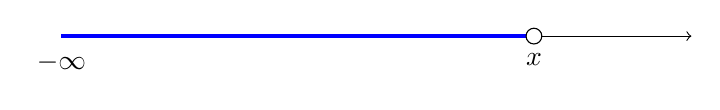
\begin{tikzpicture}
              % Eixo horizontal
              \draw[->] (-4,0) -- (4,0);
            
              % Linha vertical para representar x
              \draw[dashed] (2,-0.1) -- (2,0.1);
              % Rótulo para -∞
              \node[below] at (-4,-0.1) {$-\infty$};
              % Rótulo para x
              \node[below] at (2,-0.1) {$x$};
              % Desenhar o intervalo aberto (-∞, x)
              \draw[very thick, blue] (-4,0) -- (2,0);
              % Adicionar a bolinha aberta em x
              \draw[fill=white] (2,0) circle (0.1);
        \end{tikzpicture}
	}{
	    \Fonte{Elaborado pelo autor}
	}	
\end{figure}
Se tomarmos um $y \in \R$, com $y<x$, então podemos decompor o intervalo $(-\infty, x)$ por meio da união dos intervalos $(-\infty, y]$ e $(y,x)$, onde estão representados na figura a seguir pelas cores azul e vermelha respectivamente.\\
\begin{figure}[h!]
	\centering
	\Caption{\label{fig:boreliano-decomposto} Representação de uma decomposição do intervalo $(-\infty, x)$ na reta real}	
	\UECEfig{}{
        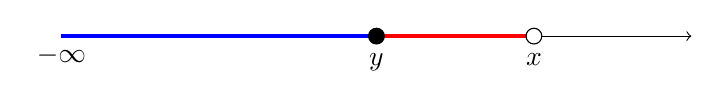
\begin{tikzpicture}
              % Eixo horizontal
              \draw[->] (-4,0) -- (4,0);
              % Linha vertical para representar x
              \draw[dashed] (2,-0.1) -- (2,0.1);
              % Rótulo para -∞
              \node[below] at (-4,0) {$-\infty$};
              % Rótulo para x
              \node[below] at (2,-0.1) {$x$};
                
              % Rótulo para a
              \node[below] at (0,-0.1) {$y$};
              
              % Desenhar o intervalo aberto (-∞, x)
              \draw[very thick, blue] (-4,0) -- (2,0);
            
              % Desenhar o intervalo aberto (a,b)
              \draw[very thick, red] (0,0) -- (2,0);
              
              % Adicionar a bolinha aberta em x
              \draw[fill=white] (2,0) circle (0.1);
              \draw[fill=black] (0,0) circle (0.1);
        \end{tikzpicture}
	}{
	    \Fonte{Elaborado pelo autor}
	}	
\end{figure}\\

É por meio dessa observação que conseguimos finalmente mostrar a equivalência adiante\\
\begin{theorem}
\label{teo:equiv-borel}
    Uma \sigal é uma de Borel  se , e somente se, é gerada por intervalos do tipo $(a,b)$ com $a,b \in \R$.
\end{theorem}

\begin{prova}
   Suponha que $(\R,\borel)$ é um espaço mensurável. 
   Sejam $a$ e $b$ números reais, com $a<b$.
   Como $a - \dfrac{1}{n} \in \R$ para todo $n \in \N$, temos que 
   $\left(-\infty, a- \dfrac{1}{n}\right) \in \R, \ \forall \ n \in \N$.
   Segue pela proposição \ref{prop:interseção-elementos-sigmas} que
   $\displaystyle \bigcap_{n = 1}^n \left(-\infty, a- \dfrac{1}{n}\right) \in \cc$.
   Afirmamos que 
   $\displaystyle \bigcap_{n \in \N} \left(-\infty, a - \dfrac{1}{n}\right) = (-\infty, a]$. 
   De fato,
   \begin{align*}
   		x \in \bigcap_{n \in \N} \left(-\infty, a - \dfrac{1}{n}\right)
   		\Leftrightarrow & x \in \left(-\infty, a - \dfrac{1}{n}\right), \ \forall n \in \N\\
   		\Leftrightarrow & x < a - \dfrac{1}{n}, \ \forall n \in \N\\
   		\Leftrightarrow & \dlim_{n \to \infty} x \leq \dlim_{n \to \infty} \left(a - \dfrac{1}{n}\right)\\
   		\Leftrightarrow & x \leq a\\
   		\Leftrightarrow & x \in (\infty, a]\\
   \end{align*}
	Logo, $(\infty, a] \in \borel$ acarretando que $(\infty, a]^c = (a, +\infty) \in \borel$.
	Observe que $(-\infty, b) = (-\infty,a] \cup (a, b)$ enquanto que $(a, b) \cup [a, +\infty)$.
	Logo, $(-\infty, b) \cap (a, +\infty) = (a,b)$. 
	Como $(-\infty, b)$ e $(a, +\infty)$ são elementos de $\borel$, segue pela proposição
	\ref{prop:interseção-elementos-sigmas} que $(a,b) \in \borel$.
	Com isso, $\borel$ pode ser gerada por intervalos do tipo $(a,b)$ com $a,b \in \R$.
   
	Suponha, reciprocamente, que $\mathcal{C}$ é uma \sigal de $\R$ que é gerada, por intervalos do tipo $(a,b)$ onde $a,b \in \R$.
	Assim, os conjuntos $A_n = (-n, b)$ são todos elementos de $\mathcal{C}$ para qualquer $n \in \N$.
	Segue, pela definição \ref{def:sigma-algebra}, que 
	$\displaystyle \bigcup_{n = 1}^\infty (-n,b) \in \mathcal{C}$.
	Só que $\displaystyle \bigcup_{n = 1}^\infty (-n,b) = (-\infty, b)$.
	Com isso, os elementos de $\mathcal{C}$ são do tipo $(-\infty, x)$.
	Portanto, $\mathcal{C} = \borel$.

\end{prova}

\section{Funções Mensuráveis}


Agora que já estamos familiarizados com o conceito de conjunto mensurável, nada mais natural que estender este conceito à funções. Trabalharemos apenas com funções de uma variável real, por enquanto.
Além disso, a partir de agora, fixemos que quando não houver menção contrária,  que $X$ será um conjunto qualquer diferente de $\varnothing$ e $\mathcal{C}$ será uma \sigal desse conjunto. 

\begin{definition}
    Uma função $f: X \to \R $ é dita $\mathcal{C}$-mensurável se, para cada $\alpha \in \R$, o conjunto $\{x \in X;\ f(x) > \alpha\} \in \mathcal{C}$.
\end{definition}

% Exemplos de Funções mensuráveis

\begin{example}[Função Constante]
\label{ex:funcao-constante}
Seja $K \in \R$ um número fixado. 
A função $f: X \to \R$ definida por $f(x) = K$, para todo $x \in \R$  é mensurável.
Para mostrarmos este fato, precisamos analisar os casos de $\alpha$.
\begin{enumerate}[label*= (\Roman*)]
\item Se $\alpha \geq K$, então o conjunto $\{x \in X; f(x) > \alpha\} = \varnothing$ uma vez que não existe $x \in X$ tal que $K = f(x) > \alpha$.
\item Se $\alpha < K$, então  o conjunto $\{x \in X; f(x) > \alpha\} = X$, pois todo $f(x) > \alpha,\ \forall x \in X$.
\end{enumerate}
Em todo caso, para todo $\alpha \in \R$, o conjunto  $\{x \in X;\ f(x) > \alpha\} \in \mathcal{C}$.
Portanto, a função constante $f$ é mensurável.

\end{example}

\begin{example}[Função Característica]
    Seja $(X, \mathcal{C})$ uma espaço mensurável e $A \in \mathcal{C}$.
    Chamamos de função característica \footnote{As vezes também é chamada  função indicadora.}
    a função $\chi_A: X \to \{0,1\}$ definida por 
    $$\chi_A(x) =\left\{\begin{array}{cc}
         1, & \textrm{\ se \ } x \in A \\
         0, & \textrm{\ se \ } x \notin A
    \end{array}\right.
    $$
Para verificar se $X_A$ é mensurável precisamos, novamente, analisar os casos de $\alpha \in \R$.
\begin{enumerate}[label*= (\Roman*)]
\item Se $\alpha > 1$, observamos que $\{x \in X; \chi_A(x)>  \alpha\} = \varnothing$, pois não há $x \in X$ tal que $\chi_A(x) > 1$.  
\item Se $ 0 <\alpha \leq 1$, então o conjunto $\{x \in X; \chi_A(x)>  \alpha\} = A$, pois apenas valores $x \in A$ tem suas imagens $\chi_A(x) = 1$ e consequentemente $\chi_A(x) \geq \alpha$.
\item  se $\alpha \leq 0$, podemos notar que o conjunto $\{x \in X; \chi_A(x)>  \alpha\} = X$, pois para qualquer que seja $x \in X$, os valores $\chi_A(x) \geq 0$.

\end{enumerate}
Em todo o caso, vemos que o conjunto $\{x \in X; \chi_A(x)>  \alpha\}$ é um elemento de $\mathcal{C}$, pois $\varnothing, X$ e $A$ são elementos de $\mathcal{C}$. Portanto, a função característica $\chi_A(x)$ é mensurável.

\end{example}

\begin{example}
\label{ex:função-continua-mensuravel}
    Considere o espaço mensurável $(\R, \borel)$. Toda função $f: \R \to \R$ contínua é Borel mensurável.
    Segundo \supercite{elon}{p.226}, se $X \subset \R$ é um conjunto aberto, então $\{x \in X; f(x) > \alpha\}$, para todo $\alpha \in \R$, é um conjunto aberto. Além disso, o teorema 2 encontrado em \supercite{elon}{p.167} nos diz que $\{x \in X; f(x) > \alpha\}$ é expresso unicamente pela união de intervalos abertos. 
    Assim, como $\R$ é um aberto, então $\{x \in \R; f(x) > \alpha\}$ é um aberto. Logo, existem intervalos abertos $I_n$ tal que $\{x \in \R; f(x) > \alpha\} = \displaystyle\bigcup_{n = 1}^\infty I_n$. Disso, $\{x \in \R; f(x) . \alpha \in \R\} \in \borel$.
    Portanto, qualquer função contínua $f: \R \to \R$ é Borel mensurável.
    \end{example}
    Lembre que ao apresentarmos a Álgebra de Borel (definição \ref{def:algebra-borel}), também mostramos na proposição \ref{prop:equiv-borel} que há mais de uma maneira de definir os borelianos.
    Para uma função $f: X \to \R$ mensurável, também podemos definir o conjunto $\{x \in X; f(x) > \alpha\}$ de várias maneiras.
    Com isso, temos a seguinte equivalência
    
\begin{theorem}
\label{teo:equiv-funcoes-mensuraveis}
    Sendo $(X,\mathcal{C})$ um espaço mensurável, para uma função $f: X \to \R$, as seguintes afirmações são equivalentes:
    \begin{multicols}{2}
        
    \begin{enumerate}[label=(\alph*)]
        \item $\forall \ \alpha \in \R, \ A_\alpha =\{x \in X;\ f(x) > \alpha \} \in \mathcal{C}$;
        \item $\forall \ \alpha \in \R, \ B_\alpha =\{x \in X;\ f(x) \leq \alpha \} \in \mathcal{C}$;
        \item $\forall \ \alpha \in \R, \ C_\alpha =\{x \in X;\ f(x) \geq \alpha \} \in \mathcal{C}$;
        \item $\forall \ \alpha \in \R, \ D_\alpha =\{x \in X;\ f(x) < \alpha \} \in \mathcal{C}$.
    \end{enumerate}
     \end{multicols}

\end{theorem}

\begin{prova}
    Dividiremos esta demonstração em três partes. A estratégia será mostrar que a afirmação $(a)$ é equivalente à afirmação $(b)$; depois que a afirmação $(c)$ é equivalente à afirmação $(d)$ ; e por fim que a firmação $(a)$ ocorre se, e somente se, a afirmação $(c)$ ocorre. 
    \begin{enumerate}[label* = (\Roman*)]
        \item Suponha a validade da afirmação $(a)$. Se $A_\alpha \in \mathcal{C}$, então $A_\alpha^c \in \mathcal{C}$, pela definição de $\mathcal{C}$-álgebra.
    Perceba que 
    $$
    x \in A_\alpha^c \Leftrightarrow   x \notin A_\alpha\\
    \Leftrightarrow  x \in X \textrm{\ e \ } f(x) \leq \alpha, \forall\ \alpha \in \R
    \Leftrightarrow x \in B_\alpha    
  $$ Assim, um elemento está em $A_\alpha^c$ se, e somente se, está em $B_\alpha$. Segue que $A_\alpha^c = B_\alpha$. Logo, $B_\alpha$ é elemento de $\mathcal{C}$.
  \item Para mostrar a equivalência entre as afirmações $(c)$ e $(d)$ utilizamos um argumento totalmente análogo à parte $(I)$, pois se $x \notin C_\alpha$, então $f(x) < \alpha$ acarretando que $x \in D_\alpha$ e vice-versa.
  \item Suponha que $A_\alpha \in \mathcal{C}$. Tome a sequência $\left(A_{\alpha -\frac{1}{n}}\right)$. Claramente, cada $A_{\alpha - \frac{1}{n}}$ é um elemento de $\mathcal{C}$, pois se $f(x) > \alpha$ para algum $x \in X$, então $f(x) > \alpha -\frac{1}{n}$. Logo, pela proposição \ref{prop:interseção-elementos-sigmas} $\displaystyle \bigcap_{n = 1}^\infty A_{\alpha -\frac{1}{n}} \in \mathcal{C}$. Além disso, note que 
\begin{align*}
    x \in \displaystyle \bigcap_{n = 1}^\infty A_{\alpha -\frac{1}{n}}
    \Leftrightarrow & x \in A_{\alpha - \frac{1}{n}}, \textrm{\ para  $n$ suficientemente grande}\\
    \Leftrightarrow & f(x)> \alpha -\dfrac{1}{n} \textrm{\ para  $n$ suficientemente grande}\\
    \Leftrightarrow &\lim_{n \to \infty} f(x) \geq \lim_{n \to \infty} \left(\alpha - \dfrac{1}{n}\right)\\
    \Leftrightarrow & f(x) \geq \alpha \\
    \Leftrightarrow & x \in C_\alpha
\end{align*}
    \end{enumerate}
Desta forma, $C_\alpha = \displaystyle \bigcap_{n = 1}^\infty A_{\alpha -\frac{1}{n}} $. Logo $C_\alpha \in \mathcal{C}$ como queríamos.

Reciprocamente, suponha que $C_\alpha \in \mathcal{C}$. Tomemos a sequência $\left(C_{\alpha + \frac{1}{n}}\right)$.
Cada elemento $C_{\alpha +\frac{1}{n}} \in \mathcal{C}$, pois para $x \in X$ devemos ter $f(x) > \beta$ para qualquer $\beta \in \R$, inclusive para $\beta = \alpha + \frac{1}{n}$. Assim, pela definição de \sigal, 
$\displaystyle \bigcup_{n = 1}^\infty C_{\alpha +\frac{1}{n}} \in \mathcal{C}$. Com isso, temos que
\begin{align*}
    x \in \displaystyle \bigcup_{n = 1}^\infty C_{\alpha +\frac{1}{n}}
    \Leftrightarrow & x \in C_{\alpha + \frac{1}{n_0}}, \textrm{\ para algum  $n_0 \in \N$ }\\
    \Leftrightarrow & f(x)\geq \alpha +\dfrac{1}{n_0}\\
    \Leftrightarrow & f(x) > \alpha \\
    \Leftrightarrow & x \in A_\alpha
\end{align*}
Assim, $\displaystyle \bigcup_{n = 1}^\infty C_{\alpha +\frac{1}{n}} = A_\alpha$. Logo, $A_\alpha \in \mathcal{C}$.
Portanto, segue de $(I), (II)$ e $(III)$ que as afirmações $(a), (b), (c)$ e $(d)$ são equivalentes.


\end{prova}

% Aritmética de Funções mensuráveis
Perceba que mesmo na presença do teorema \ref{teo:equiv-funcoes-mensuraveis} acima mostrar que uma função é mensurável é trabalhoso e repetitivo uma vez que, geralmente, é preciso verificar os casos de $\alpha$. Com isso, veremos o comportamento de operações aritméticas entre funções mensuráveis.

\begin{proposition}
\label{prop:aritmetica-uma-funcao}
Seja $f: X \to \R$ uma função real mensurável e $c \in \R$. Então as funções $cf$, $f^2$ e $|f|$ são mensuráveis. 
\end{proposition}

\begin{prova}
    \begin{enumerate}[label*=(\alph*)]
        \item Mostraremos que $cf$ é mensurável para todos os casos possíveis do número real $c \in \R$.
            \begin{enumerate}[label=(\roman*)]
                \item Se $c = 0$, então $c\cdot f(x) = 0, \ \forall \ x \in X$, ou seja, $cf$ se torna a função constante. Segue pelo exemplo \ref{ex:funcao-constante} que $cf$ é mensurável.
                \item Se $c>0$, então  dado $\alpha \in \R$, temos $cf(x) > \alpha \Leftrightarrow f(x) >\dfrac{\alpha}{c}$. 
                Logo, 
                $$
                \{x \in X; cf(x) > \alpha\} 
                = 
                \left\{x \in X; f(x) > \dfrac{\alpha}{c}\right\}
                $$
                    
                Isso ocorre para todo $\alpha$ e $f$ é mensurável, isto é, $\left\{x \in X; f(x) > \dfrac{\alpha}{c}\right\} \in \mathcal{C}$  . Logo, $cf$ é mensurável.
                \item Por fim, se $c < 0$, então existe um $z \in \R$ tal que $c = -z$.
                Assim, 
                $$cf(x) >\alpha \Leftrightarrow -zf(x) >\alpha \Leftrightarrow f(x) < -\dfrac{\alpha}{z}$$
                Assim, o conjunto $\{x \in X; cf(x) > \alpha \} = \left\{x \in X; f(x) < -\dfrac{\alpha}{z}\right\}$.
                Desta forma, o conjunto  $\left\{x \in X; f(x) < -\dfrac{\alpha}{z}\right\}  \in \mathcal{C}$ pelo  item $(d)$ do teorema \ref{teo:equiv-funcoes-mensuraveis}. Portanto,  $cf$ é mensurável.
            \end{enumerate}
            
        \item Para mostrar a mensurabilidade de $f^2$ é necessário analisar os casos de $\alpha$.
            \begin{enumerate}[label = (\roman*)]
                \item Se $\alpha < 0$, então $\{x \in X; [f(x)]^2 > \alpha\} = X$ pois $[f(x)]^2 \geq 0$ para todo $x \in X$.
                
                \item Se $\alpha \geq 0$, então para todo $x \in X$ $[f(x)]^2 > \alpha \Leftrightarrow f(x) > \pm \sqrt{\alpha}$.
                Assim, um elemento 
                $x_0 \in \{x \in X; [f(x)]^2 > \alpha\}$ se, e somente se, $x_0 \in \{x \in X; f(x)> \sqrt{\alpha}\}$ ou \linebreak $x_0 \in \{x \in X; f(x)> -\sqrt{\alpha}\}$.
                Logo, 
                
                $$\left\{x \in X; [f(x)]^2 > \alpha\right\} = \left\{x \in X; f(x)> \sqrt{\alpha}\right\}\cup \left\{x \in X; f(x)> -\sqrt{\alpha}\right\}$$
                
                Como $f$ é mensurável, por hipótese, temos que $\{x \in X; f(x)> \sqrt{\alpha}\} \in \mathcal{C}$ e \linebreak $\{x \in X; f(x)> -\sqrt{\alpha}\} \in \mathcal{C}$.
                Desta forma, usando a definição de \sigal, obtemos que  $\{x \in X; f(x)> \sqrt{\alpha}\} \cup \{x \in X; f(x)> -\sqrt{\alpha}\} \in \mathcal{C}$. Consequentemente, 
                $\{x \in X; [f(x)]^2 > \alpha\} \in \mathcal{C}$ acarretando a mensurabilidade de $f^2$.
            \end{enumerate}
            
        \item Analogamente ao item anterior, se $\alpha < 0$, $\{x \in X; |f(x)| > \alpha\} = X$.
        Por outro lado, se $\alpha \geq 0$, vemos que 
        $\{x \in X; |f(x)| > \alpha\}\{x \in X; f(x)> \alpha\} \cup \{x \in X; f(x)> -\alpha\}$.
        Assim, a mensurabilidade de $f$ acarreta na mensurabilidade de $|f|$ como desejávamos.
    \end{enumerate}
\end{prova}

% Exemplo de funções mensuráveis com aritmética
\begin{example}[Função Afim]
\label{ex:funcao-afim-mensuravel}
    Seja $a$ um número real diferente de zero. 
    A função $f: \R \to \R$ tal que $f(x) = ax$ é mensurável.
    De fato, pelo exemplo \ref{ex:função-continua-mensuravel} a função $x$ é mensurável, pois é contínua em $\R$.
    Segue pela proposição \ref{prop:aritmetica-uma-funcao} que a função $ax$ também é mensurável.
    Da maneira análoga, as funções $g,h: \R \to \R$ tais que $g(x) = x^2$ e $h(x) = |x|$ são mensuráveis.
\end{example}



\begin{proposition}
\label{prop:aritmetica-duas-funcoes}
    Sejam $f,g:X \to \R$. Se $f$ e $g$ são ambas mensuráveis, então as funções $f+g$ e $f\cdot g$ são também mensuráveis.
\end{proposition}

\begin{prova}
    
    Provaremos, primeiramente, que $f+g$ é mensurável. Ora, por hipótese, $f$ e $g$ são mensuráveis. Assim, dado $r \in \Q$, os conjuntos $\{x \in X; f(x) > r\}$ e 
        $\{x \in X; g(x) > \alpha -r\}$ são ambos elementos de $\mathcal{C}$.
        Considere o conjunto  
        
        $$H_r = \{x \in X; f(x) > r\} \cap \{x \in X; g(x) > \alpha -r\}$$
        Isto é, o conjunto dos elementos $x \in X$ tal que $f(x) 
        > r$ e $g(x) >\alpha -r$ simultaneamente.
        Com isso, afirmamos que $\{x \in X; (f+g)(x) > \alpha\} = \displaystyle \bigcup_{r \in \Q} H_r$. Com efeito, as seguintes equivalências ocorrem para um elemento $a \in X$ tomado arbitrariamente

        \begin{align*}
            a \in \{x \in X; (f+g)(x) > \alpha\} 
            \Leftrightarrow  & (f+g)(a) >\alpha \\
            \Leftrightarrow & f(a) +g(a) > \alpha \\
            \Leftrightarrow & f(a) + g(a) > \alpha -r + r\ \textrm{para } \ r \in \Q\\
            \Leftrightarrow & f(a) > r \textrm{\ e\ } g(a) > \alpha -r\ \textrm{para  } \ r \in \Q\\
            \Leftrightarrow & a \in \{x \in X; f(x) > r\} \textrm{\ e\ } a \in \{x \in X; f(x) > \alpha - r\}\  \textrm{para  } \ r \in \Q\\
            \Leftrightarrow & a \in \{x \in X; f(x) > r\} \cap \{x \in X; f(x) > \alpha - r\}\  \textrm{para  }  r \in \Q\\
            \Leftrightarrow & a \in H_r,\ \textrm{para  } \ r \in \Q\\
            \Leftrightarrow &a \in \bigcup_{r \in \Q} H_r
        \end{align*}
    Logo, a afirmação é verdadeira. Além disso, para cada $r \in \Q$, o conjunto $H_r$ é um elemento de $\mathcal{C}$, pois é  a interseção de dois elementos de $\mathcal{C}$ (proposição \ref{prop:interseção-elementos-sigmas}).
    Além disso, pela definição de $\mathcal{C}$, a coleção $\displaystyle \bigcup_{r \in \Q} H_r$ é um elemento de $\mathcal{C}$, pois $\Q$ é enumerável.
    Segue que $f+g$ é mensurável.

    Para mostrar que $fg$ é mensurável basta notar que é a composição de outras funções mensuráveis.
    De fato, dado $x \in X$, temos

    \begin{align*}
        4(fg)(x) 
        =& \ 2(fg)(x) +  2(fg)(x)\\
        =& \ [f(x)]^2 - [f(x)]^2 + 2f(x)g(x) + [g(x)]^2 - [g(x)]^2 + 2f(x)g(x)\\
        =& \ \left([f(x)]^2 + 2f(x)g(x) + [g(x)]^2\right)  - \left([g(x)]^2 - 2f(x)g(x) + [f(x)]^2\right)\\
        =& \ (f(x) +g(x))^2 - (f(x) - g(x))^2\\
        =& \ [(f+g)(x)]^2 - [(f-g)(x)]^2
    \end{align*}
    Desta maneira, $fg = \dfrac{1}{4}\left[(f+g)^2 - (f-g)^2\right]$. Segue pela proposição \ref{prop:aritmetica-uma-funcao} e a primeira parte desta demonstração que $fg$ é mensurável.
\end{prova}

\begin{example}[Função Polinomial]
\label{ex:funcao-polinomial-mensuravel}
    A função  $f:\R \to \R$ definida por $f(x) = \sum_{j = 0}^n a_jx^j$ com cada $a_j \in \R$ é mensurável.
    Com efeito, note que  $f(x) = a_nx^n + a_{n-1}x^{n-1} + \cdots + a_1x +a_0$.
    Pelo exemplo \ref{ex:funcao-afim-mensuravel} cada função $f_j:\R \to \R$ definida por  $f_j(x) = a_jx^j$ é mensurável.
    Além disso, pela proposição \ref{prop:aritmetica-duas-funcoes} a soma de funções mensuráveis é mensurável.
    Segue que $f(x) = \sum_{j = 0}^n a_jx^j$ é uma função mensurável.
\end{example}


\begin{definition}
    Seja $f: X \to \R$. Dizemos que a \textbf{parte positiva} da função $f$ é a função $f^+: X \to \R$ definida por $f^+(x) = \sup\{f(x), 0\}$.
    Semelhantemente, chamamos de a \textbf{parte negativa} da função $f$, a função $f^-: X \to \R$ definida por $f^-(x) = \sup\{-f(x), 0\}$.
\end{definition}

\begin{example}
    Seja $f: \R^* \to \R$ definida por $f(x) =\dfrac{|x|}{x}$. Se tomarmos, $x< 0$, vemos que $f(x) < 0$ sendo $f(x) = \dfrac{-x}{x} = -1$.
    Se $x>0$, então $f(x) =\dfrac{x}{x} = 1$. Assim, $f^+ = \sup\{f(x), 0\} = 1$ enquanto que $f^- = \sup\{-f(x), 0\} = -1$.
\end{example}

Neste caso, tanto a parte positiva quanto a parte negativa da função $f$ acima apresentada são funções constantes
conforme está representado na imagem a seguir

    \begin{figure}[h!]
	\centering
	\Caption{\label{fig: Gráfico da Função f(x) =|x|/x} Gráfico da Função $f(x) =\dfrac{|x|}{x}$}	
	\UECEfig{}{
	    \begin{tikzpicture}[scale=0.7]
            % \draw[black, smooth] (-3.2,-1.5) rectangle (3,3.2);
                % Cria o eixo cartesiano
                \draw[->] (-3,0) -- (4,0) node[right] {$x$};
                \draw[->] (0,-1.5) -- (0,3) node[left] {$y$};
                
                \draw[domain=-3:-0.1,very thick,variable=\x,blue] plot ({\x},{abs(\x)/\x});
                \draw[domain=0.1:3.8,very thick,variable=\x,blue] plot ({\x},{abs(\x)/\x});
            
                \draw[fill=white] (0,1) circle (0.1) node[left] {1};
                \draw[fill=white] (0,-1) circle (0.1)node[right] {-1};
            
            \end{tikzpicture}
	}{
	    \Fonte{Elaborado pelo autor}
	}	
    \end{figure}    
    Por serem constantes, já vimos que são mensuráveis. Mas e a função $f(x) =\dfrac{|x|}{x}$ é mensurável?
    A resposta é sim e para mostrarmos isso precisaremos de algumas proposições auxiliares. 
    \begin{proposition}
    \label{prop:decomposicao-da-funcao-em-partes-positiva-negativa}
        Seja $f: X \to \R$. Então $f = f^+ - f^-$ e $|f| = f^+ + f^-$.
    \end{proposition}
    \begin{prova}
            Para provar que $f = f^+ - f^-$, devemos avaliar os casos de $f(x)$. 
            Logo, se $f(x) \geq 0$, então $f^+(x) = \sup\{f(x), 0\} = f(x)$ e $f^-(x) = \sup\{-f(x), 0\} = 0$, pois $f(x) \geq 0 \Rightarrow  - f(x) \leq 0$.
            Disso, $f^+(x) - f^-(x) = f(x) - 0 = f(x)$, ou seja, $(f^+ - f^-)(x) = f(x), \ \forall x \in X$.
            Caso $f(x) < 0$, então $- f(x) > 0$. 
            Com isso,  $\sup\{f(x), 0\} = 0$ e $\sup\{-f(x), 0\} = -f(x)$.
            Segue que 
            $f^+(x) - f^-(x) = 0 - (-f(x)) = f(x)$.
            Em todo caso, $f = f^+ - f^-$.

            Analogamente, caso $f(x) \geq 0$, temos que $\sup\{f(x), 0\} = f(x)$ e $\sup\{-f(x), 0\} = 0$.
            Assim, $f^+(x) + f^-(x) = f(x)$.
            Caso, $f(x) < 0$, então $ - f(x) > 0$.
            Com isso, obtemos $\sup\{f(x), 0\} = 0$ e $\sup\{-f(x), 0\} = -f(x)$.
            Logo, $f^+(x) + f^-(x) = -f(x)$.
            Desta forma, notamos que $(f^+ + f^-)(x) = \max\{f(x), -f(x)\} = |f(x)|$.
            Portanto, $f^+ + f^- = |f|$.
    \end{prova}

    Observe que a proposição \ref{prop:decomposicao-da-funcao-em-partes-positiva-negativa} nos dá a forma das funções $f^+$ e $f^-$ de maneira implicita.
    De fato, somando as duas expressões membro a membro vemos que 
    $$f + |f| = (f^+ + f^+) - (f^- + f^-) = 2f^+$$
    Assim, podemos expressar $f^+ = \dfrac{|f| + f}{2}$.
    De maneira semelhante, podemos subtrair membro a membro e obter a expressão $f^- = \dfrac{|f| - f}{2}$. 
    Isso demonstra a proposição adiante

    \begin{proposition}
    \label{prop:identidades-das-partes-das-funcoes}
        Se $f: X \to \R$, então $f^+ = \dfrac{|f| + f}{2}$ e $f^- = \dfrac{|f| - f}{2}$.
    \end{proposition}

    \begin{theorem}
        Uma função $f: X \to \R$ é mensurável se, e somente se, suas partes negativa e positiva são mensuráveis. 
    \end{theorem}

    \begin{prova}
        Suponha que $f$ seja mensurável. Pela proposição \ref{prop:aritmetica-uma-funcao} a função $|f|$ é mensurável e pela proposição \ref{prop:identidades-das-partes-das-funcoes} as funções $f^+ = \dfrac{1}{2}(|f| + f)$ e $f^+ = \dfrac{1}{2}(|f| - f)$.
        Desta forma, as funções $f^+$ e $f^-$ são compostas por funções mensuráveis.
        Segue pela proposição \ref{prop:aritmetica-duas-funcoes} que $f^+$ e $f^-$ são mensuráveis.
        Reciprocamente, supondo que $f^+$ e $f^-$ são mensuráveis, temos pela proposição \ref{prop:decomposicao-da-funcao-em-partes-positiva-negativa} que
        $f = f^+ - f^-$. Segue, novamente pela proposição \ref{prop:aritmetica-duas-funcoes}, que $f$ é mensurável. 
    \end{prova}


    % \begin{example}
    %         Seja $f: \R \to \R$ definida por  $f(x) = (\cos x, \seno x)$.
    %         Ao analisarmos o gráfico de $f$, podemos observar que $f$ é uma circunferência de raio 1 centrada na origem conforme está ilustrada na figura abaixo
    %         \begin{figure}[h!]
    %         	\centering
    %         	\Caption{\label{fig:grafico-da-curva-circulo} Gráfico da curva $f(x) = (\cos x, \sin x)$}	
    %         	\UECEfig{}{
    %         	    \begin{tikzpicture}[scale=1.5]
    %                         % Eixos cartesianos
    %                         \draw[->] (-1.25,0) -- (2,0) ;
    %                         \draw[->] (0,-1.25) -- (0,1.75) ;
    %                         % Rótulos dos eixos
                            
    %                         \node at (1.1,-0.15) {$1$};
    %                         \node at (-0.15,1.15) {$1$};
    %                         % \foreach \x in {-1,1}
    %                         %   \draw (\x,0.05) -- (\x,-0.05) node[below right] {$\x$};
    %                         % \foreach \y in {-1,1}
    %                         %   \draw (0.05,\y) -- (-0.05,\y) node[left] {$\y$};
                            
    %                         % Gráfico da função
    %                         \draw[domain=0:2*pi,samples=100,thick,blue] plot ({cos(\x r)},{sin(\x r)});
    %                         % Legenda
    %                         \node[blue] at (1.2,1.2) {$f(x) = (\cos x, \sin x)$};
    %                     \end{tikzpicture}
    %         	}{
    %         	    \Fonte{Elaborado pelo autor}
    %         	}	
    %         \end{figure}
    %     Assim, $f^+= \sqrt{1 - x^2}$ enquanto que $f^- = - \sqrt{1 - x^2}$.
        
    % \end{example}
    
%%%%%%%%% ESPAÇOS MENSURÁVEIS
\section{Os Espaços de Funções Mensuráveis}
    O que estamos vendo até aqui é como saber se um conjunto ou uma função é mensurável, isto é, se pode ser medido.
    As vezes, teremos conjuntos "muito grandes" que podem ser medidos, mas sua medida não poderá ser expressa por um número real.
    Para solucionar este problema, apresentaremos um novo sistema.

    \begin{definition}
    \label{def:reta-estendida}
        A coleção $\xreta$ que consiste de $\R \cup \{-\infty, +\infty\}$ é chamada de \textbf{Sistema Estendido de Números Reais}.
    \end{definition}

    Este sistema é necessário por vários motivos que serão apresentados ao longo do texto. 
    Um deles, por exemplo, é a conveniência em dizer que o comprimento da Reta Real $\R$ é $+\infty$.
    Embora estejamos "adicionando" os símbolos $\pm \infty$ à reta real, vale a ressalva de que eles não são números.
    Com isso, $\xreta$ não é fechado para operações de $\R$ tais como $(+\infty) + (-\infty)$ que nem definido é.
    Dito isso, para $x \in \R$, as operações dos símbolos $+\infty$ e $-\infty$ são:

    \begin{multicols}{2}
        \begin{itemize}
            \item $(+ \infty) + (+ \infty)  = + \infty$;
            \item $x + (+ \infty) = (+ \infty) + x = + \infty$;
            \item $(- \infty) + (- \infty)  = - \infty$;
            \item $x + (- \infty) = (- \infty) + x = - \infty$;
            \item $(+ \infty)\cdot (+ \infty) =  +\infty $;
            \item $(- \infty)\cdot (- \infty) =  +\infty $;
            \item $(+ \infty)\cdot (- \infty) =  -\infty $;
            \item $(- \infty)\cdot (+ \infty) =  -\infty $.
        \end{itemize}

    \end{multicols}
    Na multiplicação, dependendo do número real, a operação diferencia-se. Assim, temos mais duas operações:
    \begin{multicols}{2}
    $$
    x \cdot (+\infty) = x \cdot (+\infty) =
    \left\{\begin{array}{cc}
          +\infty, & \ \textrm{se } x > 0\\
          0, & \ \textrm{se } x = 0\\
          - \infty, & \textrm{se } x < 0
    \end{array}\right.
    $$
    
    $$
    x \cdot (-\infty) = x \cdot (-\infty) =
    \left\{\begin{array}{cc}
          -\infty, & \ \textrm{se } x > 0\\
          0, & \ \textrm{se } x = 0\\
          + \infty, & \textrm{se } x < 0
    \end{array}\right.
    $$
        
    \end{multicols}

    Considere $\xreta$ e tomando um conjunto qualquer $\varnothing \neq E \in \borel$ , defina $E_1 = E \cup \{-\infty\}, E_2 = E \cup \{+\infty\}$ e $E_3 = E \cup \{-\infty, +\infty\}$. 
    O conjunto $\overline{\borel} = \displaystyle \bigcup_{E \in \borel} \{E, E_1, E_2, E_3\}$ é uma \sigal de $\xreta$. Com efeito, se $E \in \borel$, então é um intervalo
    Assim, as uniões dão intervalos do tipo $(-\infty,x$ ou $(x, +\infty)$ que são elementos de $\borel$.
    Pode ser que em algum momento a depender do $E$, tenhamos $(-\infty, +\infty)$.
    Este nada mais é que $\R$ que também é um elemento de $\borel$ por definição de \sigal.

    \begin{definition}
    \label{def:algebra-borel-estendida}
        A \sigal $\overline{\borel} = \displaystyle \bigcup_{E \in \borel} \{E, E_1, E_2, E_3\}$ do conjunto $\xreta$ é chamada de Álgebra de Borel Estendida. 
    \end{definition}

    Uma vez que estamos familiarizados com os conceitos de funções de valores reais mensuráveis, estamos prontos para estender este conceito para o conjunto $\xreta$.

    \begin{definition}
    \label{def:familia-funcoes-mensuraveis}
        Sendo $(X, \mathcal{C})$ um espaço mensurável, uma função de valores reais estendidos $f: X \to \xreta$ é dita $\mathcal{C}$-mensurável caso o conjunto
        $\{x \in X; f(x) > \alpha\} \in \mathcal{C}$ para qualquer que seja $\alpha \in \R$. Além disso, a família de todas as funções de valores reais estendidos de $X$ que são $\mathcal{C}$-mensuráveis é denotada por $M(X, \mathcal{C})$.
    \end{definition}

    \begin{proposition}
    \label{prop:identidade-intersecao-mais-infinito}
        Se $f \in \menfus$, então $\{x \in X; f(x) = +\infty\} = \displaystyle \bigcap_{n = 1}^\infty \{x \in X; f(x) > n\}$.
        Além disso, $\{x \in X; f(x) = +\infty\} \in \menfus$.
    \end{proposition}

    \begin{prova}
        Tome, de modo arbitrário, um elemento $a \in X$. 
        Assim, 
        \begin{align*}
            a \in \bigcap_{n = 1}^\infty \{x \in X; f(x) > n\} 
            \Leftrightarrow & a \in \{x \in X; f(x) > n\}, \ \forall n \in \N\\
            \Leftrightarrow & \forall n \in \N,\ f(a) > n\\
            \Leftrightarrow & \dlim_{n \to \infty} f(a) \geq \dlim_{n \to \infty} n\\
            \Leftrightarrow & f(a) \geq +\infty  
        \end{align*}
    Como estamos trabalhando com $\xreta$, o único elemento possível para $f(a)$ é $+\infty$.
    Logo, $f(a)  = + \infty$. Assim, tudo isso ocorre se, e somente se, $a \in \{x \in X; f(x) = +\infty\}$ como queríamos.
    Além disso, note que cada $\{x \in X; f(x) > n\} \in \mathcal{C}$.
    Segue, pela proposição \ref{prop:interseção-elementos-sigmas}, que $\displaystyle \bigcap_{n = 1}^\infty \{x \in X; f(x) > n\} \in \mathcal{C}$ acarretando que $\{x \in X; f(x) = +\infty\} \in \mathcal{C}$. 
    \end{prova}

    \begin{proposition}
    \label{prop:identidade-união-menos-infinito}
        Se $f \in \menfus$, então $\{x \in X; f(x) = -\infty\} = \displaystyle \left(\bigcup_{n = 1}^\infty \{x \in X; f(x) > - n\}\right)^c$.
        Além disso, $\{x \in X; f(x) = -\infty\} \in \menfus$.
    \end{proposition}

    \begin{prova}
        Analogamente à proposição \ref{prop:identidade-intersecao-mais-infinito} tomemos $a \in X$. 
        Desta forma, 
        \begin{align*}
            a \in \left(\bigcup_{n = 1}^\infty \{x \in X; f(x) > - n\}\right)^c
            \Leftrightarrow & a \in \bigcap_{n = 1}^\infty \left(\{x \in X; f(x) > - n\}\right)^c\\
            \Leftrightarrow & \forall \ n \in \N, a \in \left(\{x \in X; f(x) > - n\}\right)^c\\
            \Leftrightarrow & \forall \ n \in \N, a \notin \{x \in X; f(x) > - n\}\\
            \Leftrightarrow & \forall \ n \in \N, a \in \{x \in X; f(x) \leq - n\}\\
            \Leftrightarrow & \forall \ n \in \N, f(a) \leq - n\\
            \Leftrightarrow & \lim_{n \to \infty} f(a) \leq \lim_{n \to \infty} (- n)\\            
            \Leftrightarrow & f(a) \leq -\infty\\            
            \Leftrightarrow & f(a) = -\infty\\            
            \Leftrightarrow & a \in \{x \in X; f(x) = -\infty\}            
        \end{align*}
        
    Ora, cada $\{x \in X; f(x) > - n\} \in \mathcal{C}$.
    Assim, por definição de \sigal, temos que $\bigcup_{n = 1}^\infty \{x \in X; f(x) > - n\} \in \mathcal{C}$ e também 
    $\left(\bigcup_{n = 1}^\infty \{x \in X; f(x) > - n\}\right)^c \in \mathcal{C}$.
    Portanto, $\{x \in X; f(x) = -\infty\} \in \mathcal{C}$. 
    \end{prova}

    \begin{theorem}
    \label{teo:condição-de-mensurabilidade}
        Um função $f: X \to \xreta$ é mensurável se, e somente se, os conjuntos 
        $A = \{ x \in X; f(x) = +\infty\}$ e $B = \{x \in X; f(x) = -\infty\}$
 são elementos de $\mathcal{C}$ e a função $h: X \to \R$ definida por
 
 $$
 h(x) = \left\{\begin{array}{cc}
     f(x), & \textrm{\ se } x \notin A\cup B  \\
      0,& \textrm{\ se } x \in A\cup B
 \end{array}\right.
 $$
 é mensurável.
 \end{theorem}
\begin{prova}
    Ora, $f \in \menfus$. Logo, pelas proposições \ref{prop:identidade-intersecao-mais-infinito} e \ref{prop:identidade-união-menos-infinito}, $A,B \in \mathcal{C}$.
    Assim, tome $\alpha \in \R$ com $\alpha \geq 0$, então os elementos de $\{x \in X; h(x) > \alpha\}$ são os elementos de $\{x \in X; f(x) > \alpha\}$ que não estão em $A$, pois $h$ tem contradomínio $\R$.
    Logo, $\{x \in X; h(x) > \alpha\}$.
    Caso, $\alpha < 0$, então os elementos de $\{x \in X; h(x) > \alpha\} = \{x \in  X ; f(x) > \alpha\} \cup B $.
    Com isso $h$ é mensurável.

    Por outro lado,  se $A,B$ são elementos $\mathcal{C}$ e $h$ é mensurável, então
    $$\{x \in X; f(x) > \alpha\} = \{x \in  X ; h(x) > \alpha\} \cup A $$
    quando $\alpha \geq 0$, e 
    $$\{x \in X; f(x) > \alpha\} = \{x \in  X ; h(x) > \alpha\} - B $$
    quando  $\alpha < 0$.
    Portanto, $f$ é uma função mensurável.
\end{prova}

por consequência dos teoremas \ref{prop:aritmetica-uma-funcao} e o teorema \ref{teo:condição-de-mensurabilidade} vemos que se $ f \in M(X,\mathcal{C})$, então as funções $cf, f^2, |f|, f^+$ e $f^-$ também são elementos de $M(X, \mathcal{C})$.
% Faltam os dois últimos ressultados ainda. Falar com o orientador.
%%%%%%%%%% Espaços de Medida

\section{Espaços de Medida}

Nas subseções anteriores, nós trabalhos com conjuntos e com funções mensuráveis, isto é, que podem ser medidas de alguma forma.
Nesta subseção, nos preocuparemos em definir e trabalhar com funções de um espaço mensurável $(X, \mathcal{C})$ que daremos o nome de "medida".
Tais funções são induzidas pela nossa concepção de comprimento, área, volume, etc.
Dito isso, para trabalhamos com medidas primeiro retomaremos alguns resutlados sobre sequência de conjuntos.

\begin{definition}
\label{def:sequência-crescente-decrescente-de-conjuntos}
    Uma sequência de conjuntos $(A_n)$ é dita \textbf{crescente} se $A_n \subseteq A_{n+1}$ para todo $n \in \N$.
    Caso tenhamos $A_n \supseteq A_{n+1}$ para todo $n \in \N$, dizemos que a sequência  de conjuntos é \textbf{decrescente}.
\end{definition}

\begin{proposition}
\label{prop:sequencia-crescente-conjuntos-resultado-A_n}
Seja $(E_n)$ uma sequência crescente de conjuntos. Se $(A_n)$ é tal que $A_1 = E_1$ e $A_n = E_n - E_{n -1}$ para todo $n > 1$, então:
\begin{enumerate}[label* = (\roman*)]
    \item $A_n$ é uma sequência disjunta;
        \footnote{Lembre que uma sequência disjunta significa que $A_i \cap A_j = \varnothing$ para todo $i \neq j$}
    \item $E_n = \displaystyle \bigcup_{j = 1}^n A_n$;
    \item $\displaystyle \bigcup_{j = 1}^\infty E_n = \displaystyle \bigcup_{j = 1}^\infty A_n$;
\end{enumerate}
\end{proposition}

\begin{prova}
    Para provar $(a)$ precisamos mostrar que para todo $n,m \in \N$ se $m \neq n$, então $A_n \cap A_m = \varnothing$.
    Lembre que $A - B = A\cap B^c$ para quaisquer conjuntos $A$ e $B$.
    Desta forma, como a interseção entre conjuntos é associativa e comutativa temos que
    \begin{align*}
        A_m\cap A_n =& (E_m - E_{m -1}) \cap (E_n - E_{n -1})\\
        =& (E_m \cap E_{m -1}^c) \cap (E_n \cap E_{n -1}^c)\\
        =& (E_m \cap E_n) \cap ( E_{m -1}^c\cap E_{n -1}^c)\\
        =& (E_m \cap E_n) \cap \left( E_{m -1}\cup E_{n -1}\right)^c\\
    \end{align*}
    Com isso, se $m > n$, então $E_n \subseteq E_m$ e $E_{n-1} \subseteq E_{m-1}$, pois $(E_n)$ é uma sequência crescente.
    Além disso, $E_m^c \subseteq E_{m -1}^c$ e $E_m \cap E_m^c = \varnothing$.
    Segue que
    $$
    (E_m \cap E_n) \cap \left( E_{m -1}\cup E_{n -1}\right)^c =
    (E_m) \cap E_{m -1}^c = 
    \varnothing
    $$
    Caso tenhamos $m < n$ temos $E_m \subseteq E_n$ e $E_{m-1} \subseteq E_{n-1}$.
    Segue analogamente que 
    $$
    (E_m \cap E_n) \cap \left( E_{m -1}\cup E_{n -1}\right)^c =
    (E_n) \cap E_{n -1}^c = 
    \varnothing
    $$
    Em todo caso, $A_m \cap A_n = \varnothing$ para todo $m \neq n$.

    Provaremos o item $(b)$ por indução sobre $n$.
    Como $(E_n)$ é crescente, temos que $E_1 \subseteq E_2$.
    Com isso, temos que 
        \begin{align*}
            \bigcup_{j = 1}^2 A_j = A_1 \cup A_2= & E_1 \cup (E_2 - E_1)\\
            = & E_1 \cup (E_2 \cap E_1^c)\\
            = & (E_1 \cup E_2) \cap (E_1 \cup E_1^c)\\
            = & (E_1 \cup E_2) \cap \mathcal{C}\\
            = & (E_1 \cap E_2)
            = E_2  
        \end{align*}
    Suponha que exista um $k \in \N$ tal que $\displaystyle \bigcup_{j = 1}^k A_j = E_k$.
    Mostraremos que $\displaystyle \bigcup_{j = 1}^{k+1} A_j = E_{k +1}$ também é verdadeira.
    Com efeito, 
    \begin{align*}
        \bigcup_{j = 1}^{k+1} A_j =& \left(\bigcup_{j = 1}^{k} A_j\right) \cup A_{k+1}\\
        =& E_k \cup A_{k +1}\\
        =& E_k \cup (E_k - E_{k+1})\\
        =& E_k \cap E_{k+1}\\
        =& E_{k+1}\\
    \end{align*}
    Segue, pelo método da indução finita, que $\displaystyle \bigcup_{j = 1}^n A_j = E_n\ \forall n \in \N$.

    Por fim, $(c)$ é um resultado imediato, pois $ x \in \displaystyle \bigcup_{j = 1}^\infty E_j$ se, e somente se, 
    existe um $n_0 \in \N$ tal que $x \in E_{n_0}$. 
    Pelo item $(b)$, isso só ocorre se $x \in \displaystyle \bigcup_{j = 1}^{n_0}A_j$.
    Mas isso é equivalente à dizer que existe um $k$ com $1\leq k\leq n_0$ tal que $x \in A_k$.
    Como $k \in \N$ isso acontece se, e somente se, $x \in A_k$ para algum $k \in \N$.
    Portanto $x \in \displaystyle \bigcup_{j = 1}^\infty A_j$.
\end{prova}

\begin{proposition}
\label{prop:sequencia-decrescente-conjuntos-resultado-A_n}
Seja $(F_n)$ uma sequência decrescente de conjuntos. 
Se $(E_n)$ é tal que $E_n = F_1 - F_n$ para todo $n \in \N$, então $(E_n)$ é crescente e 
$\displaystyle \bigcup_{j = 1}^\infty E_n = \displaystyle F_1 - \bigcup_{j = 1}^\infty F_n$.
\end{proposition}

\begin{prova}
    Queremos mostrar que $(E_n)$ é crescente, isto é, $E_n \subseteq E_{n+1}$ para todo $n \in \N$.
    Tome $x \in E_n$. Logo, $x \in F_1$ e $x \notin F_n$, por construção.
    Como $(F_n)$ é decrescente, $F_{n} \supseteq F_{n+1}$. 
    Assim, $x \notin F_n \Rightarrow x \notin F_{n+1}$.
    Com isso, $x \in F_1$ e $x \notin F_{n+1}$.
    Segue que $x \in E_{n+1}$ e que $E_n \subseteq E_{n+1}$ para qualquer $n \in \N$ como queríamos.
    Além disso, um elemento $a \in \displaystyle \bigcup_{n \in \N} E_n$ se, e somente se,
    $a \in \displaystyle \bigcup_{n \in \N} (F_1 - F_n)$.
    Isso é equivalente a dizer que existe um $n_0 \in \N$ tal que $a \in F_1 - F_{n_0}$.
    Correspondentemente, $ a \in F_1$ e existe um $n_0 \in \N$ tal que $x \notin F_{n_0}$.
    Isso só ocorre se $x \in F_1$, mas $x \notin \displaystyle \bigcup_{n \in \N} F_n$.
    Portanto, $\displaystyle \bigcup_{j = 1}^\infty E_n = \displaystyle F_1 - \bigcup_{j = 1}^\infty F_n$.
\end{prova}

\begin{definition}
\label{def:medida}
    Uma medida é uma função $\mu: (X, \mathcal{C}) \to \xreta$ tal que satisfaz as seguintes condições:
    \begin{enumerate}[label* = (\roman*)]
        \item $\mu(\varnothing) = 0$;
        \item $\mu(E) \geq 0, \ \forall A \in \mathcal{C}$;
        \item Se $(A_n)$ é uma sequência disjunta de elementos de  $\mathcal{C}$, então 
        $\displaystyle\mu\left(\bigcup_{n = 1}^\infty A_n\right) = \sum_{n = 1}^\infty\mu(A_n)$.
        
    \end{enumerate}
\end{definition}

Ou seja uma medida é uma função não negativa que é contavelmente aditiva.
Além disso, o valor de $\mu$ pode ser igual à $+\infty$ para algum conjunto $A \in \mathcal{C}$.
Quando temos que $\mu(E) < +\infty$ para qualquer que seja o conjunto $E \in \mathcal{C}$, dizemos que temos uma medida finita.


% Exemplos de medida
\begin{example}
    Seja $X$ um conjunto e $\mathcal{C}$ a sigma álgebra formada por todos os subconjunto de $X$.    
    Defina $\mu_1, \mu_2:\mathcal{C} \to \xreta$ pondo $\mu_1(A) = 0$ para qualquer  $A \in \mathcal{C}$ e 
    $\mu_2$ é  pondo 

$$\mu_2(A) = \left\{\begin{array}{cc}
0, & \textrm{\ se \ } A = \varnothing \\
+\infty,& \textrm{\ se \ } A \neq \varnothing
\end{array}\right.$$
Sendo definidas dessa forma, as funções $\mu_1$ e $\mu_2$ são medidas.
De fato, em ambas as condições \textit{(i)} e \textit{(ii)} são trivialmente satisfeitas.
Para a condição \textit{(iii)}, temos que qualquer sequência disjunta $(A_n)$ acarretará que

$$\mu_1\left(\bigcup_{n = 1}^\infty A_n\right) = 0 = \sum_{n = 1}^\infty 0 = \sum_{n = 1}^\infty \mu_1(A_n) $$
Para $\mu_2$ temos dois casos possíveis.
Se  $\displaystyle \bigcup_{n = 1}^\infty A_n  = \varnothing$, então $\mu_2\left(\displaystyle \bigcup_{n = 1}^\infty A_n\right) = 0$. Entretanto isso ocorre somente se $A_j = \varnothing$ para todo $j \in \N$.
Logo, 

$$\sum_{n = 1}^\infty \mu_2(A_n) = \sum_{n = 1}^\infty \mu_2(\varnothing) = \sum_{n = 1}^\infty 0 = 0$$
Caso $\displaystyle \bigcup_{n = 1}^\infty A_n  \neq  \varnothing$, conseguimos observar que os termos da sequência $(A_n)$ só podem ser de dois tipos ou $A_j = 0$ ou $A_j = +\infty$ para algum $j \in \N$. Com isso,  $\mu_2\left(\displaystyle \bigcup_{n = 1}^\infty A_n\right) = +\infty$.

Ademais, na soma $\displaystyle \sum_{n = 1}^\infty \mu_2(A_n)$ só teremos soma dos termos $0 + (+ \infty)$ ou $(+\infty) + (+\infty)$.
Desta forma, $\displaystyle \sum_{n = 1}^\infty \mu_2(A_n) = \sum_{n = 1}^\infty \mu_2(A_n) = +\infty$.
Portanto $\mu_1$ e $\mu_2$ são medidas.
\end{example}



% Unidade de Medida Concentrada em p
\begin{example}[Unidade de Medida Concentrada em $p$]
\label{ex:medida-concentrada-em-p}
    Seja $(X, \mathcal{C})$ um espaço mensurável tal como no exemplo $a$ e $p$ um elemento de $X$.
    Defina $\mu: \mathcal{C} \to \xreta$  como sendo


$$\mu(A) = \left\{\begin{array}{cc}
0, & \textrm{\ se \ } p \notin A \\
1, & \textrm{\ se \ } p \in A 
\end{array}\right.$$


Então $\mu$ é uma medida.
Verdadeiramente, observe que $p \notin \varnothing$, ou seja, $\mu(\varnothing) = 0$.
Trivialmente, tem-se $\mu(A) \geq 0,\ \forall A \in \mathcal{C}$, pela construção de $\mu$.



\end{example}

% Medida de contagem
\begin{example}
    Seja $X = \N$ e $\mathcal{C}$ sendo o conjunto das partes de $\N$. 
para $A \in \mathcal{C}$, definimos $\mu(A)$ por meio da sua cardinalidade, isto é, se $A$ é finito, então $\mu(A)$ é quantidade de elementos de $A$. Caso contrário, $\mu(A) = +\infty$.

\end{example}



% Teorema


\begin{theorem}
\label{teo:operacoes-com-medidas-1}
	Seja $\mu$ uma medida definida sobre uma \sigal $\mathcal{C}$.
	Se $A$ e $B$ são elementos de $\mathcal{C}$ e $A \subset B$, então $\mu(A) \leq \mu(B)$
	Se $\mu(A) < +\infty$, então $\mu(A-B) = \mu(A) - \mu(B)$.
\end{theorem}

\begin{prova}
	Suponha que $A \subset B$, então $A = B \cup (B - A)$ e $A \cap (B - A) = \varnothing$. Segue pela propriedade $(ii)$ que 
	
	$$\mu(B) = \mu(A) + \mu(B-A)$$
 Lembre que $B-A = B\cap A^c$. Como $A \in \mathcal{C} \Rightarrow A^c \in \mathcal{C}$.
 Além disso, como $B \in \mathcal{C}$ temos que $ B\cap A^c$ consequentemente $B - A \in \mathcal{C}$.
 Assim, como $\mu$ é uma medida e $B-A \in \mathcal{C}$, temos que $\mu(B-A) \geq 0$.
 Segue pela definição da relação de $\geq$ que $\mu(B) \geq \mu(A)$.
 Observe que se $\mu(A) < \infty$, temos que 

	$$\mu(B) = \mu(A) + \mu(B-A) 
 \Leftrightarrow \mu(B) - \mu(A) =  \mu(B-A)
 $$
Como desejávamos.
\end{prova}

\begin{proposition}
\label{prop:limite-sequencia-crescente}
Seja $\mu$ uma medida definida sobre uma \sigal $\mathcal{C}$.
Se $(E_n)$ é uma sequência crescente de $\mathcal{C}$, então $\mu\left(\displaystyle \bigcup_{n = 1}^\infty E_n\right) = \dlim_{n \to \infty} \mu(E_n)$.
\end{proposition} 

\begin{prova}
    Ora, se $\mu(E_n) = +\infty$ para algum $n \in \N$ ambos os lados da equação acima são $+\infty$.
    Desta forma, vamos supor que $\mu(E_n) < +\infty$ para todo $n \in \N$.
    Com isso, vamos construir uma sequência $(A_n)$ pondo $A_1 = E_1$ e $A_n = E_n - E_{n-1}$ para qualquer $n>1$.
    Então pela proposição \ref{prop:sequencia-crescente-conjuntos-resultado-A_n}, $(A_n)$ é uma sequência disjunta, temos $E_n = \bigcup_{j = 1}^n A_j$ e $\bigcup_{j = 1}^\infty E_j = \bigcup_{j = 1}^\infty A_j$.
    Como $\mu$ contavelmente aditiva, 
    $$\mu\left(\bigcup_{n = 1}^\infty E_n\right)
    =\mu\left(\bigcup_{n = 1}^\infty A_n\right)
    = \sum_{n = 1}^\infty \mu(A_n)
    = \lim_{m \to +\infty}\sum_{n = 1}^m \mu(A_n)$$
    Pelo teorema \ref{teo:operacoes-com-medidas-1} vemos que $\mu(A_n) = \mu(E_n) - \mu(E_{n - 1 })$ para $n > 1$.
    Assim, 
    
    \begin{align*}
        \lim_{m \to +\infty}\sum_{n = 1}^m \mu(A_n)
        =&
        \lim_{m \to +\infty}(\mu(A_1) + \mu(A_2) + \cdots +\mu(A_m))\\
        =&
        \lim_{m \to +\infty}(\mu(E_1) + \mu(E_2 - E_1) + \cdots +\mu(E_m - E_{m-1}))\\
        =&
        \lim_{m \to +\infty}(\mu(E_1) + \mu(E_2) - \mu(E_1) + \cdots +\mu(E_m) - \mu(E_{m-1}))\\
        =&
        \lim_{m \to +\infty}(\mu(E_1) - \mu(E_1) + \mu(E_2)  + \cdots  - \mu(E_{m-1}) +\mu(E_m) )\\
        =&
        \lim_{m \to +\infty} \mu(E_m)
    \end{align*}
    Segue que $\mu\left(\displaystyle \bigcup_{n = 1}^\infty E_n\right) = \dlim_{n \to \infty} \mu(E_n)$.




% Note que $H_2 = A_2 - A_1$ e $H_3 = A_3 - A_2$. Logo, $H_1 \cup H_2 \cup H_3$
% Assim, 

% % \begin{align*}
%     \bigcup_{n = 1}^4 H_n =&
%     \bigcup_{n = 1}^4 (A_n - A_{n-1})\\
%     =&
%     \bigcup_{n = 1}^4 \left(A_n \cap (A_{n-1})^c\right)\\
%     =&
%     \left(A_1 \cap (A_{1-1})^c\right)\\
    
% \end{align*}


\end{prova}

\begin{proposition}
Seja $\mu$ uma medida definida sobre uma \sigal $\mathcal{C}$.
Se $(B_n)$ é uma sequência decrescente de $\mathcal{C}$ e $\mu(B_1) < +\infty$, então 
$\mu\left(\displaystyle \bigcap_{n = 1}^\infty B_n\right) = \dlim_{n \to \infty} \mu(B_n)$.
\end{proposition} 
\begin{prova}
    Defina uma sequência $(T_n)$ de elementos de $\mathcal{C}$ pondo $T_n = B_1 - B_n$ para qualquer que seja $n \in \N$.
    Pela proposição \ref{prop:sequencia-decrescente-conjuntos-resultado-A_n}, $(T_n)$ é crescente.
    Assim, aplicando o a proposição \ref{prop:limite-sequencia-crescente} temos que 
    $$
    \mu\left(\bigcap_{n \in \N} T_n\right) = \lim_{n \to +\infty} \mu(T_n)
    $$
    Usando o teorema \ref{teo:operacoes-com-medidas-1}, obtemos
    $$
    \lim_{n \to +\infty} \mu(T_n) = \lim_{n \to +\infty} [\mu(B_1) - \mu(B_n)] = \mu(B_1) - \lim_{n \to +\infty} \mu(B_n)
    $$
    Segue pela proposição \ref{prop:sequencia-decrescente-conjuntos-resultado-A_n} que 
    $$
    \lim_{n \to +\infty} \mu(T_n) = \mu(B_1) - \mu\left(\bigcap_{n \in \N} B_n\right)
    $$
    Combinando as duas equações obtemos que
    \begin{align*}
        \mu(B_1) - \lim_{n \to +\infty} \mu(B_n) = \mu(B_1) - \mu\left(\bigcap_{n \in \N} B_n\right)
    \end{align*}
    Portanto, $\displaystyle \lim_{n \to +\infty} \mu(B_n) = \mu\left(\bigcap_{n \in \N} B_n\right)$
\end{prova}

% Espaços de Medida

\begin{definition}
    Dizemos que uma tripla ordenada $(X, \mathcal{C}, \mu)$ constituída por um conjunto $X$, uma \sigal $\mathcal{C}$ desse conjunto e uma medida $\mu$ sobre o espaço mensurável $(X, \mathcal{C})$ é um espaço de medida.
\end{definition}

Uma vez que já foram bem explorados os espaços mensuráveis e os espaços de medida, nosso objetivo neste capítulo é medir 
